\documentclass[conference]{IEEEtran}
% \IEEEoverridecommandlockouts
% The preceding line is only needed to identify funding in the first footnote. If that is unneeded, please comment it out.
\usepackage{cite}
\usepackage[utf8]{inputenc}
\usepackage[T1]{fontenc} % hrvatski
\usepackage{currvita} % hrvatski
\usepackage{amsmath,amssymb,amsfonts}
\usepackage{algorithmic}
\usepackage{graphicx}
\usepackage{textcomp}
\usepackage{xcolor}
\usepackage[super]{nth}
\def\BibTeX{{\rm B\kern-.05em{\sc i\kern-.025em b}\kern-.08em
    T\kern-.1667em\lower.7ex\hbox{E}\kern-.125emX}}
\begin{document}

\title{Generating song lyrics using recurrent neural networks\\
{\footnotesize Project for the course \textit{Neural Networks} at Faculty of
Electrical Engineering and Computing, University of Zagreb}
}

\author{
\IEEEauthorblockN{Ena Car}
\IEEEauthorblockA{Ena.Car@fer.hr}
\and
\IEEEauthorblockN{Pavao Dužević}
\IEEEauthorblockA{Pavao.Duzevic@fer.hr}
\and
\IEEEauthorblockN{Damjan Grubelić}
\IEEEauthorblockA{Damjan.Grubelic@fer.hr}
\and
\IEEEauthorblockN{Josipa Kaselj}
\IEEEauthorblockA{Josipa.Kaselj@fer.hr}
\and
\IEEEauthorblockN{Magdalena Šimunec}
\IEEEauthorblockA{Magdalena.Simunec@fer.hr}
\and
\IEEEauthorblockN{Eva Šmuc}
\IEEEauthorblockA{Eva.Smuc@fer.hr}
}

\maketitle

\begin{abstract}
This document is a project report for the Neural Networks course at Faculty of
Electrical Engineering and Computing in Zagreb. It describes an implementation
of a recursive neural network which is used for generating song lyrics based
on given set of song lyrics.
\end{abstract}

\begin{IEEEkeywords}
RNN, neural networks, generating song lyrics
\end{IEEEkeywords}

\section{Introduction}
Writing meaningful lyrics has always been a challenge even to the best of
songwriters. Since more and more jobs are being automated, especially now with
the rise of popularity of various machine learning methods, there is also an
initiative aimed at computers writing songs.
The goal is to feed a model with lyrics of existing songs and then to use it for
generating new lyrics. Those generated song lyrics aren't supposed to be
word-for-word equal to those used for training the model. Still, it wouldn't be
sensible having it generate random words, either. The goal is having the model 
memorize the lyrics of the songs it is trained on (motifs) and then combine them
\textit{sensibly}, i.e. having the model memorize "relationships" between the
words through their relative order.
In this project, it is being done using recursive neural networks (RNN), which
are able to take in account previous outputs when generating new one, thus
adding temporality. 
The models have been trained on several subsets of the "150K Lyrics Labeled with 
Spotify Valence" dataset from \textit{kaggle.com}.

\section{Existing solutions and brief literature overview}

\subsection{Automatic Rap Lyrics Generation}
Variation of RNN called LSTM architecture creates a better language model than a regular RNN. \cite{b1}
According to Potash, Romanov and Rumshisky, Long Short-Term Memory (LSTM) language model
produces better lyrics than a baseline model. They attempted to piece together lyrics for a specific artist, but
their model was limited in generating lyrics for a genre. As a result of training their model with sets of lyrics, they
noticed corresponding rhyming words. \vspace{2.5mm}

Another example of A Rap Lyrics Generator was developed by Nguyen and Sa \cite{b2}.
They used database of approximately 40000 existing rap lyrics. After failure to get profound results when using 
linear-interpolated trigram model approach, they shifted to a quadgram model. Also, they succeeded to generate sentences 
that rhyme with each other. At the end, generator worked decently, but the content of the lyrics did not relate to a specific theme.

\subsection{Automatic Generation of Poems}
Wishful Automatic Spanish Poet was the first generating program for poems which used artificial intelligence and natural language
generation techniques together. The whole system of WASP is based on a forward reasoning ruled-based system.
Users were asked for inputs which were then used as seeds and results recieved were not very efficient in generating lyrics \cite{b3}.

\subsection{Rhyme Detection}
Hirjee and Brown have developed a probabilistic model and in addition to it they have built up a rhyme detection tool based on that model \cite{b4} \cite{b5}.
Tool analyzes phoneme patterns in words and model is trained on a set of lyrics that were manually annotated for rhyming words.

\subsection{Classification of Lyrics}
Mayer, Neumayer and Rauber used rhyme and style features to classify and process lyrics \cite{b6}. 
They followed the fact that a rhyme is two words that when spelt sound similar and generally used it for words at the end of verses.

\subsection{Natural Language Processing and Lyrics Generation}
With basic natural language processing tools, song lyrics can be analysed by using a Naive Bayes classifier. Mahedero, Cano and Martinez used that to 
identify languages. Also, they used it for classification based on themes and to search for similarities between them. 
The languages which were used for the experiment: English, Spanish, German, French and Italian. Given results were approximately 94\% accurate.
The conclusion they came to is that the identification of languages was easier task compared to the others.

\section{Solution implemented by the project team} % mozda bolji naslov?
Since generating the lyrics requires memorizing word ordering so that lyrics
make sense, RNNs have been used, as that class of neural networks is better for
memorizing sequences. Sequences used as RNN inputs can be words as well as
characters. In this project, the word-based model has been used, so that
all generated lyrics use existing words and the RNN doesn't have to memorize
character ordering inside the words on top of word order.

\subsection{Choosing the right dataset}
The lyrics needed for training such model can be scraped using the webscrapers
on lyrics websites, downloaded using a Python API like \textit{lyricsgenius} or
downloaded as a readily available dataset. With the latter being the simplest
method of the three, yet equally suitable, the project team opted for the
"150K Lyrics Labeled with Spotify Valence" dataset because of its exhaustiveness
which provides a simple way to extract almost any arists' lyrics and  offers
diversity of songs and genres. Since it is too big to be processed on the
project team's machines, only the first 200 lyrics with more than 60\% English
words in them have been used for training the most of the models.

\subsection{Preprocessing the dataset}
Since the lyrics texts often contain additional info that is not part of actual
song lyrics (like the chorus tag or the name of the artist performing the
next verses) and since such tags are most commonly enclosed in square brackets,
everything inside square brackets has been removed from the lyrics to
reduce cluttering with info that may not be correct in generated lyrics and
would interfere with memorizing relationships of words and motiffs.

However, another kind of interference was made in
order to memorize line endings. The "word" \textit{endl} has been added to the
end of each line in order to help with rhyming and breaking lines of
generated songs in meaningful places.

After adding the \textit{endl}, each word from the dataset has been stripped of
punctuation and converted to lowercase. Each word has been mapped to a unique
number that would be used as network input.

Those numbers (tokenized words) have been grouped into sequences of 
\textbf{up to} $n$ lines, i.e. verses. The sequences have been padded to the
length of the longest sequence with zeros. The last number in each sequence
would later be expected output for the input which is the rest of the sequence.

\subsection{Building the models}
Three different architectures of neural network have been used in order to determine which one would provide the best results.
Basic network architecture consists of an input layer, one or multiple hidden layers and an output layer.

First architecture consists of one hidden SimpleRNN layer, which is a fully-connected RNN where the output is to be fed back to input.

Second architecture has an LSTM as a hidden layer and a Dropout layer in order to prevent overfitting.

The third and most complex architecture consists of one Bidirectional LSTM layer, a Dropout layer in order to prevent overfitting, LSTM layer and two densely-connected NN layers.

The softmax function is used as the activation function in the output layer of all the neural network models 
since they predict a multinomial probability distribution. 
Adam optimizer was used since it achieves good results faster than classical stochastic gradient descent optimizer.

\subsection{Training the models}
Each model was trained for a period of 20, 50, 80 and 110 epochs in order to determine when underfitting and overfitting happens. 

\subsection{Generating the lyrics}
The lyrics are being generated line by line, with tokenized words from $n$
previous lines as the input for the model. The first line doesn't have previous
lines, but a seed text may be added instead. Model then predicts for each unique
word from the corpus how likely it is to appear next. That word is added to
the song and then the model makes a new prediction for the next word with the
last one added to the input.

Since lyrics tend to be repetitive, especially after overfitting, the model may
fall in loop predicting the same lyrics over and over. That's why the
genrating function explicitly prevents two lines starting with the same word
by picking the second word that is the most likely to appear. It also reduces
the impact of overfitting by memorizing the exact lyrics from dataset:

Any song with identical words at the start of two close lines cannot be exactly
reproduced by the generator.

Number of lines is randomly selected from the same distribution as the numbers
of lines of the lyrics in the dataset.

\subsection{Evaluation of the generated lyrics}
The measure of the model fitness during the training has been "how well the
model reproduces the lyrics it was given". However, the goal isn't to reproduce
the same lyrics that already exist, but to generate \textit{new} meaningful songs. 

Measuring how good some lyrics are is a problem of its own, because it's highly
subjective and hardly quantifiable. There are ways to analyze the structure of
generated lyrics and the distribution of the words \cite{b7}, but with such a
diverse dataset, there isn't a proper point of reference and that still isn't 
sufficient to tell if the lyrics really are good.

So for the evaluation, apart from how the lyrics looked to the project team, an
online tool "made by songwriters" was used as they may have more proficiency in
analysis --- The Lyric Assessor.

The Lyric Assessor is calibrated using the lyrics of 295 songs that are cited by songwriters as being examples of well-crafted songs. It scores the lyrics with a number ranging form -5 to 5. 
Scores above zero (maximum = 5) indicate that the lyrics are linguistically more like lyrics often mentioned as archetypically well-crafted songs by songwriters.
Scores below zero (minimum = -5) indicate that the lyrics are linguistically less like lyrics often mentioned as archetypically well-crafted songs by songwriters.
The Lyric Assessor has an accuracy of approximately 80\%. It uses computational linguistics to compare lyrics with a corpus of songs regarded as "well-crafted" by songwriters and with a corpus of songs not so regarded by songwriters.

\section{Project results}
The generated lyrics can be found in the Appendix \ref{APDX}.
Scores by the Lyric Assessor for the generated lyrics  are given in Table 
\ref{scores}, which is plotted in ``Fig.~\ref{fig}''.

% converted the table according to the template:
\begin{table}[htbp] % "insert figures and tables after they're cited in the text"
\caption{The Lyric Assessor scores depending on model architecture and training time}
\begin{center}
\begin{tabular}{|c|c|c|c|}
\hline
\textbf{Number of}&\multicolumn{3}{|c|}{\textbf{Architecture}} \\
\cline{2-4} 
\textbf{epochs} & \textbf{\textit{SimpleRNN}}& \textbf{\textit{SimpleLSTM}}& \textbf{\textit{BiLSTM}} \\
\hline
20 & -0.9 & 1.9 & -4.3 \\ % inserting body of the table
50 & 1.7 & 2.1 & 1.6 \\
80 & -0.3 & 2.6 & 3.1 \\
110 & 1.3 & 0.5 & 0.8 \\
\hline
\end{tabular}
\label{scores}
\end{center}
\end{table}

\begin{figure}[htbp]
\centerline{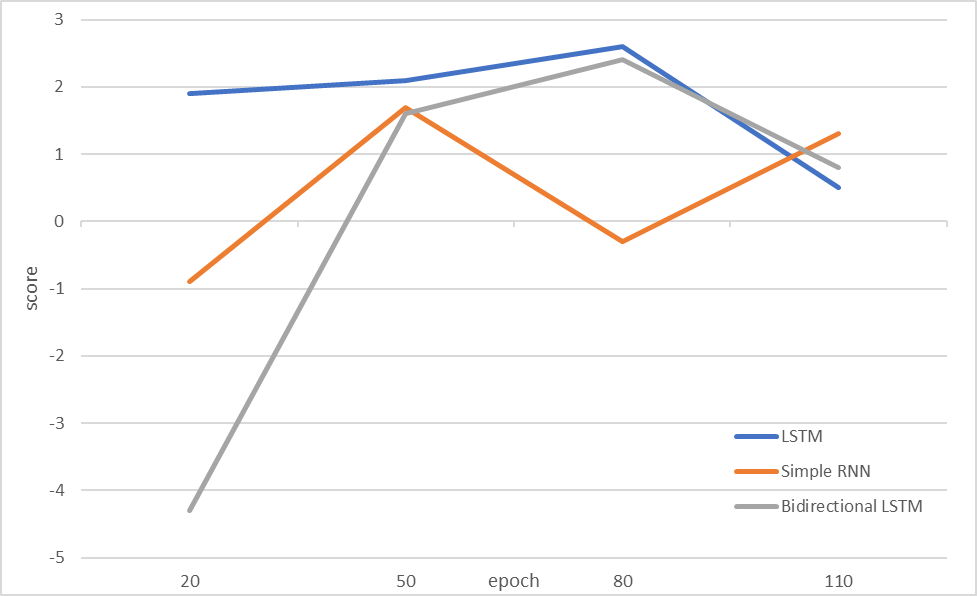
\includegraphics[width=0.5\textwidth]{scoregraph.png}}
\caption{Score graph}
\label{scoregraph}
\end{figure}

\subsection{Comparison by architecture}
Comparison of the lyrics generated after 80 epochs by three different models:
\ref{LSTM80}, \ref{RNN80}, \ref{HID80}.
When comparing the results, we look at how well the song is crafted in terms of syntax and semantics, and the similarity to what is generally perceived as 'well written' lyrics. 
Simple RNN architecture generated lyrics where the verses lack syntactic sense and words following one another seem very random (\ref{RNN80}). 
The most complex architecture based on Bidirectional LSTM generated lyrics which demonstrated overfitting. After training the model for 80 epochs, it generated song lyrics asssembled from verses identical to existing songs from the dataset.
Architecture with one hidden LSTM layer and regularisation provided satisfactory results(\ref{LSTM80}). The generated lyrics improved in terms of syntax and semantics when compared to the ones generated by Simple RNN model. The words do not seem as random, while overfitting is avoided due to a balance of simpler architecture and right amount of epochs used for training the model.

\subsection{Comparison by epoch}
It can be concluded from the scoring, 
that for Simple LSTM results keep getting better up until 80 epochs. Training this particular model for more than 80 epochs decreases the score.
The more complex model based on Bidirectional LSTM seems to achieve the best score - 3.1 for 80 epochs. This makes sense since the song lyrics 
generated for this model after 80 epochs are almost identical to verses provided in the dataset, so The Lyric Assessor is more likely to consider 
this song archetypically well-crafted.

Accuracy of the models during training can be seen in ``Fig.~\ref{fig}''.

\begin{figure}[htbp]
\centerline{
\includegraphics{fig1.png}}
\caption{Accuracy of the models}
\label{fig}
\end{figure}

\subsection{Comparison by artist}
To better show how generated lyrics reflect the dataset a model is trained on,
a simple LSTM model was trained for 110 epochs on a dataset consisting of only
Boney M.\ref{A1} songs, and it was repeated on Iron Maiden's songs \ref{A2}.

Both generated lyrics contain recognizable words from the artists' songs. Their
style was harder to replicate. Some of the words even form whole lines identical
to those in the songs, which is a sign of overfitting. 
%Dylanometer

\section{Comparison with existing solutions}
For comparison, we have used an already existing project with a character-based approach with mild modifications.

The important difference from our solution is that this network must learn words and the order of the letters to get a meaningful word.
Also, has to learn the order between the words.

The project uses the Sequential model which is one way of creating deep learning models. 
It is convenient to use when each layer has only one input tensor and one output
tensor. The Sequential model is defined by passing a list of layers to the Sequential
constructor.

Firstly, words are presented as vectors that need to be evaluated to match
something meaningful and that is done by calling embedding. Embedding turns positive integers
into dense vectors of fixed size. 

After that, Gated Recurrent Units (GRU) is used to remember
a certain number of previous words in a clever way (rnn\_units). GRU is used as a closing mechanism in RNN (something like LSTM, but with fewer parameters). 

Finally, a dense layer is a deeply connected layer
from its preceding layer which works for changing the dimension of the output by
performing matrix-vector multiplication and gives information about the most probable word that
is expected.

We used similar parameters and architectures as with our model for comparison. 
The most noticeable disadvantage is that some words do not make sense, that is, we can call them ''garbage''.

An important parameter when generating lyrics is \textbf{temperature}. Low temperature will produce predictable results, but with 
higher temperature lyrics will become more creative. That can be seen in 
\ref{Sequential512_1024_200}, which is a more complex model than
\ref{Sequential256_1024_200}, but contains less words from the songs and less
correctly spelled words in general, but better recovers from the overfitting loop.

\section{Conclusion}
Generally, the most complex architecture: the LSTM with hidden layers overfits
most quickly and training it on a bigger dataset may produce good results in the
same number of epochs. Simple LSTM is faster. It produces better results than
simple RNN model.

Generally,
the resulting lyrics generator doesn't produce completely random lyrics nor does
it really create lyrics that make sense. Given the limited resources and time,
the results are as expected because the results from the literature aren't much
better.

Further work based on this project might include developing a metric that would
measure lyrics fitness. That may also enable using reinforcement learning which
could lead to better results.

Another approach that may yield better results would be using GPT instead of RNN.

% apostrofi - mogli smo ih pretvoriti u prave riječi bez apostrofa
% smanjenje broja memoriziranih riječi u tokenizeru po učestalosti
% probati bez n-grama? Fiksan broj riječi umjesto linija?

%dodati da bi nam alternativa bila brojanje slogova ili riječi ili nekaj 
% u zaključak - kaj bi se još moglo


\section{Appendix}\label{APDX}

\subsection{Simple LSTM - 20th epoch}\label{LSTM20}
i'm running for my life \\
and won't you believe it \\
how can you need it \\
\\
i will never rest the system's sympathy \\
california california california california \\
it's merilee \\
since you been gone \\
\\
i know you want to run far away from one more \\
but i don't know what you want to get tooken \\
and you think of you were not \\
there's a fire in the belt of hercules \\
don't let up what you want me any slack \\
who cares about you \\
i thought i did \\
man i need you i need you \\
\\
you know you know what you told me \\
no is the house we used to live in \\
this is a place and you gotta real too \\
and the way i feel me \\
i gotta ask to you you \\
but i do you i need you like the questions ones though \\
\\
t i p \\
man you don't need to get to you \\
you know my song \\
no fist is needed when you call \\
\\
just because of you boy \\
oh boy \\
i know you should hate me \\
but you rearrange me \\
coming in my ear \\
baby \\
i've got a hand for you \\
'cause i wanna run with you \\
won't you let me run with you \\
\\
have fun again \\
i want you to have fun \\
just like little children \\
like the little children \\
know how they have fun \\

\subsection{Simple LSTM - 50th epoch}\label{LSTM50}
i'm going and i can't say you \\
i know that i have to do \\
'till i want to be \\
'cause i got it so much \\
it's not right to you \\
 \\
i know you want to run far away from one more \\
but now these days are gone i'm not so self assured \\
now i find i've changed my mind \\
get to be \\
 \\
there's a chink of light there's a burning wick \\
what you say your arms and you can't feel \\
f*** it like our first time i get off the mess \\
just like you feel a lot and zip up an dog \\
the sun is sinking low \\
when i was raised different \\
what you feel baby \\
 \\
have fun again \\
i want you to have fun \\
just like little children \\
like the little children \\
know how they have fun \\
 \\
i need you \\
but you don't know what is not \\
for you my love \\
to escape \\
i'm why not \\
when i want to be in a man \\
so pleasant and heavenly when you \\
and you can give me i'm tell you \\
 \\
we keep 'em hotter than the fire are good \\
i cried in the sack with the flower \\
you can't put the same old time \\
and i don't have to pretend \\
since you're gone \\

\subsection{Simple LSTM - 80th epoch}\label{LSTM80}
it's a man in a glass house tonight \\
and i only want to treat you right \\
i love i love you true \\
 \\
love is all that's left in the end \\
my house and i'll take it \\
so i have got a lot of what you got to \\
keep us from the \\
and let the time i come to a man \\
when i'm out and in a speed of your eyes and the way \\
 \\
i would not believe it like these faces talk of shit by \\
y'all happened shining with a crime \\
and the hood ask about about a body so \\
stand out here in his band on your eyes \\
what's on my ass so hard and all \\
i don't quit like a phoenix \\
 \\
never never love love love \\
all the time \\
don't mind \\
you got me i need it \\
 \\
t i p \\
y'all wrong with you a way and forget \\
i know i need a man i can act \\
but i got a kid and i can always done \\
 \\
when i can see the switch man out in the freight yard \\
waving his lights at my train \\
red fir stopping my heart from beating \\
green in the air \\
 \\
you gave me my man \\
and his little thing to make me like make me were it \\
but i have like a lot of love in store \\
once in the lot of the sky \\
the sky is the mountains \\
while the system tell me by \\
cause i see the star is in \\

\subsection{Simple LSTM - 110th epoch}\label{LSTM110}
it's a man in the glass house than the days is for a lie \\
 \\
look at the only the shape don't go \\
and i don't get to the places that i want to go \\
to find some back \\
my time \\
don't think i can't stop \\
 \\
and you seek with you \\
i can't think you standing by the yes \\
they're gonna show you see my \\
think i stay in the night \\
say the f*** we used to live in \\
where the girls \\
you know i love things \\
just like little children \\
 \\
like the little children \\
know how they have fun \\
meanwhile back at the ranch \\
i think you are my condition \\
 \\
and you seek i love you \\
like you walk for the life you \\
see the first man \\
when i get out and i get my shit \\
i miss her lips \\
and i feel the unity \\
you can't believe the hook \\
no shit tonight \\
oh oh oh oh oh \\
 \\
i want you to have fun \\
have fun again \\
you asked me to prove my skills \\
then i showed ya \\
the clock ticks down \\
seems i wait the same old places \\
 \\
i was a brand new world and they've loves me \\
just like you and not get to get up with me \\
and you say that i will live my soul \\
so never never love never never love \\
 \\
never never love love love \\
all the time \\
don't mind \\
i can't think you if you can take me \\
you don't know whatcha got till it gone \\
but you don't know what you want and this ain't how it should be \\
why you gotta be so cold \\
pleasing you seems impossible \\
girl you know you're black to the bone \\

\subsection{Simple RNN - 20th epoch}\label{RNN20}
when you've hearts \\
 \\
and i'm all over my tears \\
but i walk away \\
i wish i could bring it back \\
wish i could take it back \\
 \\
now i was wrong \\
and i'm so that he got that i love you \\
i got that i got that i got that i got that \\
what i only like let you want to you \\
so i hope that take everything \\
don't think that i've got to only so empty here \\
 \\
keep it in the family \\
the real world's outside your door \\
you can't take it in you \\
it's here for long \\
and you can't be happy \\
oh why still \\
he said if i could even that i was th' way that comes out this rest \\
 \\
now i can see you don't belong \\
if i open all the day to make that mind \\
and i'll take the taste to be it's far \\
the man was treating me the feeling but at the mountain \\
 \\
they looked people the water \\
is the voices wake his toy \\
and heaven has its ways \\
love will do on a doubt \\
to work through the blaze \\
doubling up the stacks \\
he said if god lives by the gun \\
\subsection{Simple RNN - 50th epoch}\label{RNN50}
so i said \\
i don't had a calculator \\
to know i'm gonna see you later \\
and i don't need a secretary \\
for the next door all make it a rose to my mind \\
you get new more of sleep \\
a futile attempt to uphold your claim \\
as i don't even myself but i want to do so many not believe some sleep \\
\\
this fire's down they put mind by the good move \\
your heart i was the day \\
when i know what i saw \\
but i don't care how i was mine \\
i wish that each reasons \\
on the salt lakeline \\
casey jones \\
got another poppa \\
my special time \\
\\
why would you ever get \\
it was \\
so old are love yes you push you weak \\
i'd keep it in my list \\
and if there's what the way was mine \\
oh you can hear \\
\\
slow to me for the only way oh \\
to the harp and his back \\
but you've almost gonna before to fly \\
all i need you listen \\
we shall come on a him \\
his child was mine \\
the looked is on in the mouth \\
make a blanket with my baby \\
through a good little dream \\
\subsection{Simple RNN - 80th epoch}\label{RNN80}
so i won't clean up on the cry \\
i'll find you \\
a place when you're not low \\
it's everything makes it \\
\\
you are everything \\
everything is you \\
oh you are everything \\
say i might like her thing when you find \\
\\
now i'm standing inside outside which is the right side \\
i'm standing the left side \\
the flat earth december \\
when your body you'll be \\
and i'll get big broken bones \\
that then the day seems always just want go on \\
\\
i'd let it pass you on by a world \\
i can't hide what's in here \\
standing going alone \\
a moment echoing yeah \\
every gonna miss that he's see my little \\
and you are singing \\
\\
all the way of the side \\
make room in here are world \\
makes it crawl while get by now \\
where i play her in the grou ou ou ou ound \\
a travesty starin' at me ee \\
\\
old glass houses ivory towers \\
they flash like a sun and meet with fun \\
just stop a blood above \\
fadin' night \\
if my boss finds through the crowd \\
\\
no i'm it in the sky \\
and i was cold my heart so melting or oh \\
he's it in the way \\
people will dat a man is a sigh \\
\\
won't be the here that see with my lies \\
i found you melt inside him \\
i'm falling in your own \\
baby to read it up \\
\\
and the same not you begun \\
every simple lies that it's they \\
in a feather \\
as i don't get paid \\
oh pretty please \\
was all alone \\
\\
all within \\
the public enemy's the man that goes new acts blind \\
searching in a girl of the basement \\
holding the verdict is a heart that i could got a time to your heart \\
i open his little just \\
do to your phone \\
\\
they never met with you babe \\
how it's hard for me for the next train he can rock glass a left \\
for the station and \\
he stepped into the cabin \\
my life seems so man \\
go on the world \\
\\
i'm just miles on a car \\
just miles on a car \\
i only need a map of where you are \\
they'll never be right fun \\
\\
when i was arrested i was dressed in black \\
they put me on a train and they took my mind \\
and he'll think you don't you \\
no i tried on about them when they go out our hearts cryin' \\
more love i know that's all we need \\
know what we've seen \\
\subsection{Simple RNN - 110th epoch}\label{RNN110}
i don't need a calculator \\
to know i'm gonna see you later \\
and i don't need a secretary \\
so where the sun of alone \\
best things take love \\
if you're anywhere \\
made me one last kiss \\
and they're just miles on a car that \\
just up twenty in my time \\
but i only wish i get ever \\
\\
you i love you \\
i'm a liar \\
so left me \\
i let you go unselfishly \\
'cause everyone needs time \\
\\
ktulu ktulu so bad \\
if you want to hear \\
with another day \\
on your feet \\
move it to the rhythm \\
\\
just miles on a car \\
i only need a map of where you are \\
they'll never be a place that is too far \\
and you and the change out it's me \\
you got out \\
i'd give to laugh \\
i'm gonna go my pack is tonight \\
i knew now you see driving you \\
\\
you got that winging for your head \\
shut your mouth \\
but he went away \\
the invader will split \\
so they were at the right in which man \\
and i got if i die \\
flip flop and fly \\
i don't care if i die \\
don't ever leave me \\
\subsection{LSTM (Hidden Layer) - 20th epoch}\label{HID20}
i might not know what love is \\
but i know what it ain't \\
\\
you are everything \\
everything is you \\
oh you are everything \\
you're so f****n' special \\
i wish i was special \\
\\
but i'm a creep i'm a weirdo \\
what the hell am i doing here \\
the radio was his toy \\
was a beautiful day out in santa cruz \\
they were feelin' so good it shoulda been a crime \\
come all night to that memphis beat \\
\\
i'm not looking back \\
but i want to look around me now \\
time stands still \\
see more of the people \\
and the places that surround me now \\
\subsection{LSTM (Hidden Layer) - 50th epoch}\label{HID50}
i never knew \\
the likes of you \\
\\
extraordinary thing \\
you're all going to die down here \\
get out \\
that every day i just wanna give you \\
much more love \\
i'm warped and it was thing that a piece of sunshine \\
and there's a for sale sign on a little house \\
i saw just about a mile or so from here \\
but i've always been the kind for pullin' up the stakes \\
it's ain't never been like me to put down roots \\
\\
you're too near me nasty boy girl \\
me i'm gonna ever happen \\
stand up and i'm back in the race \\
nothing is going to stop me \\
i wasn't born to fail \\
i'm taking the inside rail \\
\\
all the odds against me \\
in the two horse race \\
you're so won't know \\
no ambition just existing sorrow breaks a good man down \\
\\
i remember all the good times when the world was ours to flame \\
then she left me took the sunshine every night wind speaks her name \\
can't stop loving can't stop living there's no answer to be found \\
no ambition just existing sorrow breaks a good man down \\
\\
i remember all the good times when the world was ours to flame \\
then she left me took the sunshine every night wind speaks her name \\
\subsection{LSTM (Hidden Layer) - 80th epoch}\label{HID80}
i name it exalted \\
a restrained shaman \\
\\
mother russia \\
dance of the czars \\
hold up your heads \\
be proud of what you are \\
now it has come \\
freedom at last \\
turning the tides of history \\
and your past \\
\\
mother russia \\
dance of the czars \\
hold up your heads \\
be proud of what you are \\
now it has come \\
freedom at last \\
turning the tides of history \\
and your past \\
\subsection{LSTM (Hidden Layer) - 110th epoch}\label{HID110}
i just can't go on livin' life as i do \\
comparing each boy to you babe \\
no no they just won't do \\
\\
chorus \\
all you know versus all you don't \\
i know just find a gun \\
i'll give them a state a state of unconsciousness \\
retribution no solution constitution \\
discrimination through the nation raining hatred \\
\\
keep it in the family \\
i'm the thing that you most fear \\
i don't keep it in the family \\
don't even try to tell me what you think is right \\
when to you blacks are ni****s and jews are k***s \\
and you expect to be taken seriously \\
but your actions they're more than curiously \\
juvenile you emulate what you hate \\
you love me \\
\\
and there's always something more that i should tell you \\
more lost that i am found \\
so i'm trying to clear my head so i'll be \\
the box was cool and the band was prime \\
they made it back up front to their seats just in time \\
a place to hell for bait for a while \\
\\
as i would tell you weh di ruggu ruggu use \\
dat's what jr gong him use \\
you're gonna laugh when you're down and out boy \\
i'm gonna laugh when you're on that lonesome ride \\
\\
back all the way to china in a police car from japan oh yeah \\
sitting in the backseat crying \\
where's your pride \\
and slap yourself on the back \\
before you tell me what you heard \\

\subsection{Boney M.}\label{A1}
time for me of all right \\
sing a happy morning \\
\\
all the people \\
'cause the people are leavin' \\
when the people believin' \\
they didn't get a lovers in the middle of the night \\
it's their out \\
but he ever how to you \\
he was a steppenwolf and with a smile she died \\
\\
no no no one at all \\
now ma ma ma \\
ma baker \\
she taught her four sons \\
\\
by the rivers of babylon there we sat down \\
ye eah we wept when we remembered zion \\
all the way of angels \\
o come let us adore him \\
christ the lord \\
\\
sing choirs of angels \\
music isn't somewhere \\
they gathered all around him \\
to see him and adore \\
\\
this day will live forever \\
oh my lord \\
my lord \\
he is a personation \\
there came great jubilation \\
la la de da la la de da \\
all you gotta say is la de da \\
\subsection{Artist 2}\label{A2}
i am a fugitive being hunted down \\
like game \\
so we'll be in \\
our way to kiss \\
to be the one that will ends \\
\\
can you see what they do \\
they are grinding us down \\
who are the fear of your need \\
and night my blood where you see \\
\\
i am a fugitive being hunted down \\
like game \\
but i am the chosen one \\
i'm not a man i'm a dead time \\
for my hand i'll be you i will know i'll give me back \\
\\
i can't begin to understand the lies to run \\
you're the same in my father \\
and i'll be alright \\
just a dream is inside \\
\\
i feel they would chosen the woman we will have a done \\
or that i heard it to me \\
please tell me now what love is \\
i'm not too born \\
that i know what i want \\
and i don't i know i'm not so there \\
\\
when i can know what to know \\
i'm gonna gonna let it on my hell \\
i feel i hope that i like the chance to \\
all the things that we cherish and love \\
nothing left but to face this all on my own \\
cause i am the chosen one \\

\subsection{Sequential - (256, 1024) - 30th epoch, 200 lyrics}\label{Sequential256_1024_200}
I'm gonna be ke when you sing along \\
With me block jaybird, \\
Why should you sacrifice \\
If you're not my enemy anymore \\
There's a hard habit to break \\
Such a hard habit to break \\
Such a hard habit to break \\
Such a hard habit to break \\
Such a hard habit to break \\
Such a hard habit to break \\
Such a hard habit to break \\
Such a hard habit to break \\

\subsection{Sequential - (512, 1024) - 30th epoch, 200 lyrics}\label{Sequential512_1024_200}
I'll be the goou under thas way a dream about me \\
I'm yours 'til I die \\
So in love \\
So in love \\
So in love \\
So in love \\
\\
I've got to go away? \\
If the sun should do \\
I drigiou don't old me close and hold me fartasy empty alone we two \\
\\
Man, it's telling jokes \\
In a nightclub \\
\\
Pearl's a singer \\
She starts there was a time when you let me go \\
(Let me go) \\
\\
I don't know why you stay \\
'Cause you don't owe me nothing \\
But you give it to me "I'm farmain the baby please don't go \\
Cause if nobody hears that I rave. \\
The pony sty \\
The darktown surr that I wanted was yours, \\
Making my wart a feel of your bird \\
From California to London town, \\
I will hold it down, \\
I promise so baby please don't go \\
Cause if nobody hears that tree fall down, \\
Does it make a sound? \\
And am I even here if I'm alone \\
\\
And there's nothing, I can broke my heart, but what of it \\
Say, its only a carvas look into her faces \\
The one light \\
I see la vie en rose \\
\\
When you kiss my ways it blows \\
Everybody knows that the dou \\


\begin{thebibliography}{00}
\bibitem{b1} P. Potash, A. Romanov, and A. Rumshisky, GhostWriter: Using an LSTM for Automatic Rap Lyric Generation. In: \emph{Proceedings of the 2015 Conference on Empirical Methods in Natural Language Processing}, 2015.
\bibitem{b2} H. Nguyen, and B. Sa, Rap Lyrics Generator, unpublished, 2009.
\bibitem{b3} H. Manurung, G. Ritchie, and H. Thompson, Towards a Computational Model of Poetry Generation. In: \emph{Proceedings of AISB Symposium on Creative and Cultural Aspects and Applications of AI and Cognitive Science}, pp. 79-86, April 2000.
\bibitem{b4} H. Hirjee, and D. Brown, Using automated rhyme detection to characterize rhyming style in rap music, 2010.
\bibitem{b5} H. Hirjee, and D. Brown, Rhyme analyzer: An analysis tool for rap lyrics. In: \emph{Proceedings of the 11th International Society for Music Information Retrieval Conference}, 2010.
\bibitem{b6} R. Mayer, R. Neumayer, and A. Rauber, Rhyme and Style Features for Musical Genre Classification by Song Lyrics. In: \emph{ISMIR 2008, \nth{9} International Retrieval, 14-18 September, 2008, Drexel University, Philadelphia, PA, USA}.
\bibitem{b7} H. Gill, D. Lee1 and N. Marwell, Deep Learning in Musical Lyric Generation: An LSTM-Based Approach. In: \emph{Yale Undergraduate Research Journal, Vol 1.1}, September 2020.

\end{thebibliography}

\end{document}
